% !TeX root = ../tesis.tex

\chapter*{Background and Motivation}
\addcontentsline{toc}{chapter}{\protect\numberline{}Background and Motivation}	  		% Comment if you don't want the introduction to appear on the table of content. It will not have a number
\label{chapter:intro}

% this file is called up by thesis.tex
% content in this file will be fed into the main document


Optical metasurfaces are bidimensional arrays of metallic/dielectric nanostructures ---known as meta-atoms--- specifically tailored to behave in a way no found in nature when illuminated at a specific wavelength in the visible light regime \cite{khan_optical_2022,gonzalez-alcalde_large_2020}. Depending on the physical properties of the meta-atoms, that is, their material, size, shape, and orientation and distribution within the bidimensional array \cite{kim_plasmonic_2019,khan_optical_2022}, a metasurface  allows to shape at will the  spatial optical response of the system \cite{chen_review_2016}, thus suiting them for a variety of applications in fields such as Spectroscopy \cite{khan_optical_2022}, Color Structuration \cite{gonzalez-alcalde_large_2020} Communications \cite{chen_review_2016} and Sensing \cite{estevez_trends_2014,jain_noble_2008,khan_optical_2022,chen_review_2016,kim_plasmonic_2019}. In the last decades, the interest of optical metasurfaces in medical disciplines has increase due to  the need for sensitive, fast, low-cost and easy-to-use technologies \cite{estevez_trends_2014,kim_plasmonic_2019}, like metasurfaces with plasmonic (metallic) meta-atoms used as contrasting agents for Bioimaging  \cite{kim_plasmonic_2019} and as free-label biosensors returning real-time measurements \cite{estevez_trends_2014,kabashin_plasmonic_2009,khan_optical_2022}.

Metasurfaces designed for biosensing typically consist of a nanostructurated substrate with compatible microfluidics illuminated with a white light source and a light recollection system, allowing for scattering or extinction measurements, followed by an spectrometer \cite{estevez_trends_2014,feuz_improving_2010}. One particular kind of  biosensing-amied metasurfaces consist in plasmonic meta-atoms, which are employed since light can be confined at nanometric scales, yielding an improvement in the sensitivity of various detection techniques \cite{khan_optical_2022}. The light confinement is the result of the meta-atom's Localized Surface Plasmon Resonance (LSPR) being excited at the meta-atom's interface with its surroundings, which occurs when the electromagnetic fields couple to the free electrons of the plasmonic structure \cite{chen_review_2016,kim_plasmonic_2019,estevez_trends_2014}.  Since the LSPR is material and geometry dependent, a variety of plasmonic metasurfaces have been designed \cite{feuz_improving_2010,kabashin_plasmonic_2009,qiu_dual_2020,svedendahl_refractometric_2014} ---each with its own benefits and disadvantages \cite{chen_review_2016,estevez_trends_2014}--- as those shown in  Fig. \ref{fig:Back}, all of which are plasmonic metasurfaces consisting of gold (Au) meta-atoms on a glass substrate but with different geometries and distributions within the metasurface.  For example, Feuz et. al. \cite{feuz_improving_2010} employed a short-range ordered metasurface of nanoholes to sense protein binding events in real-time [Fig. \ref{sfig:back:a}], while  Kabashin et. al. \cite{kabashin_plasmonic_2009} measured  changes of the refractive index of the media embedding an ordered metasurface of plasmonic nanorods [Fig. \ref{sfig:back:b}].  Metasurfaces with simpler geometries and distributions can be used  for biosensing as well, as shown by Svedendahl et. al. \cite{svedendahl_refractometric_2014}, who sensed protein binding events with a short-range ordered metasurface of nanospheres [Fig. \ref{sfig:back:d}], or by  Qiu et. al. \cite{qiu_dual_2020}, who employed a disordered metasurface of nanospheres to detect selected DNA sequences from Severe Acute Respiratory Syndrome Coronavirus 2 (SARS-CoV-2) [Fig. \ref{sfig:back:c}].

\begin{figure}[h!]
\centering
\hspace*{-3.5em}%
\begin{tikzpicture}[scale = .9]
	  \node at (0,0) {  \includegraphics[width = \textwidth]{background.png}};
		\node at (-8.3,4.15) {  \begin{subfigure}{.2\textwidth}\caption{ }\label{sfig:back:a}\end{subfigure}};
		\node at (-2.3,4.15) {  \begin{subfigure}{.2\textwidth}\caption{ }\label{sfig:back:b}\end{subfigure}};
		\node at (-2.3,-1) {  \begin{subfigure}{.2\textwidth}\caption{ }\label{sfig:back:c}\end{subfigure}};
		\node at (5.2,4.15) {  \begin{subfigure}{.2\textwidth}\caption{ }\label{sfig:back:d}\end{subfigure}};
\end{tikzpicture}
  \vspace*{-1.75em}
  \caption[Backgrounds]{Examples of biosensing-aimed plasmonic metasurfaces. \textbf{a)} Short-range ordered metasurface of nanoholes in a Au film [Scanning Electron Microscopy (SEM) image and meta-atom schema] and real-time measurements of the LSPR redshift due to protein binding events; images extracted and modified from \cite{feuz_improving_2010}. \textbf{b) } Reflectivity minimum shift of an ordered metasurface of Au nanorods (SEM image and schema in inset) as a function of the refractive index change of the media embedding the metasurface; images extracted and modified from \cite{kabashin_plasmonic_2009}. \textbf{c)} Schematics of a disordered metasurface of Au nanospheres designed for SARS-CoV-2 detection and the LSPR response of its meta-atom: Thermoplasmonic and plasmonic sensing; image extracted from \cite{qiu_dual_2020}. \textbf{d)} Experimental and theoretical results for the ellipsometric parameter $\Delta$ as a function of the incident wavelength when a short-ranged ordered metasurface of Au nanospheres (SEM image) is illuminated by a  non-polarized white light as shown in the setup diagram; extracted and modified from \cite{svedendahl_refractometric_2014}.
  }
\label{fig:Back}
\end{figure}

The design of plasmonic metasurfaces undergo several stages, but it can be roughly divided in two: its fabrication process and its theoretical behavior. On the one hand, the fabrication process relies on a variety of methods depending on the desired meta-atom's physical properties and distribution, for example, metasurfaces suited for biosensing are commonly  fabricated by lithography technics, like electron beam lithography (ordered array) or hole-mask colloidal lithography  (ordered and disordered arrays) \cite{estevez_trends_2014}, thermal annealing of thin metallic films (disordered arrays)  \cite{qiu_dual_2020} and chemical growth-methods \cite{estevez_trends_2014,kabashin_plasmonic_2009}. On the other hand, the theoretical behavior estimates the optical response of the metasurface either by numerical methods, like the Finite Element Method (FEM) \cite{feuz_improving_2010} or the Finite Differences Time Domain \cite{qiu_differential_2015} ---both employed either for periodic arrays or for meta-atoms with complex geometries--- or by analytical models, like the Thin Island Theory \cite{svedendahl_refractometric_2014,bedeaux_optical_2004}, the Dipolar Model \cite{barrera1991optical} ---both developed for disordered bidimensional arrays of nanospheres on a substrate--- or the Maxwell Garnett Model ---originally developed for 3D colloidal systems of spheres \cite{sihvola_electromagnetic_2008}--- modified to describe bidimensional systems of non-spherical meta-atoms \cite{oates_characterization_2011} as done by Kabashin et. al. \cite{kabashin_plasmonic_2009}. It is stressed that such calculations returns the optical response of the metasurface under ideal conditions as, for example, perfect geometrical shapes of the meta-atoms, perfect periodicity or even perfect deposition on the substrate supporting the meta-atoms.

Biosensing-aimed metasurfaces are supported on a substrate and immersed in an aqueous superstate \cite{estevez_trends_2014} and its theoretical behavior is usually analyzed under the assumption that the meta-atoms are perfectly supported on the substrate and perfectly embedded in the superstate  \cite{kabashin_plasmonic_2009,qiu_differential_2015,barrera1991optical,svedendahl_refractometric_2014,bedeaux_optical_2004} nevertheless, a partial embedding of the meta-atoms into the substrate can arise experimentally depending on the parameters of the fabrication process  \cite{meng_anisotropic_2015,moirangthem_enhanced_2012}. The partial embedding of the meta-atoms is inversely related to the sensing area of the metasurface in the superstrate, thus limiting its performance, but it is also directly related to the washability of its meta-atoms due to the coupled microfluidics. Therefore, the partial embedding of the meta-atoms is a physical feature that can be optimized to design a long-lasting and sensitive metasurface for biosensing, yet, few publications on partially embedded nanustractures can be found even for simple geometries like nanospheroids. In Fig. 

\begin{figure}[h!]\centering
\hspace*{-.795\textwidth}
    \begin{subfigure}{1.075\textwidth}\caption{\hfill }\label{sfig:inc:1}\end{subfigure}%
  	\begin{subfigure}{.19\textwidth}\caption{\hfill }\label{sfig:inc:2}\end{subfigure}\\[-1.225em]
  	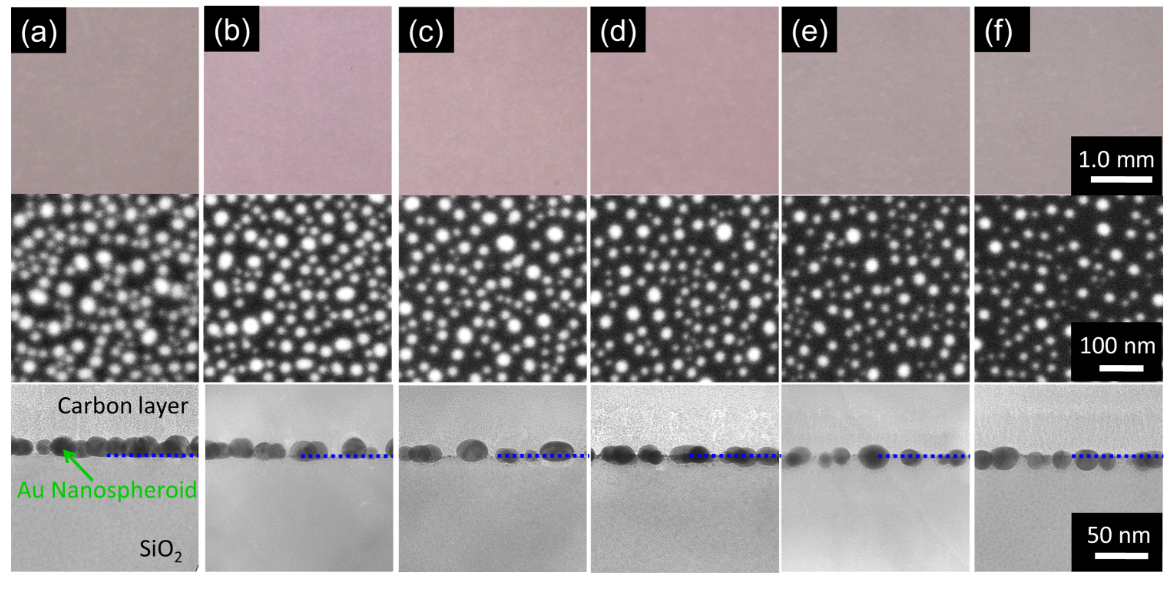
\includegraphics[width = .6\textwidth]{Meng/embedded.png}%
  		\hspace*{1em}
  	 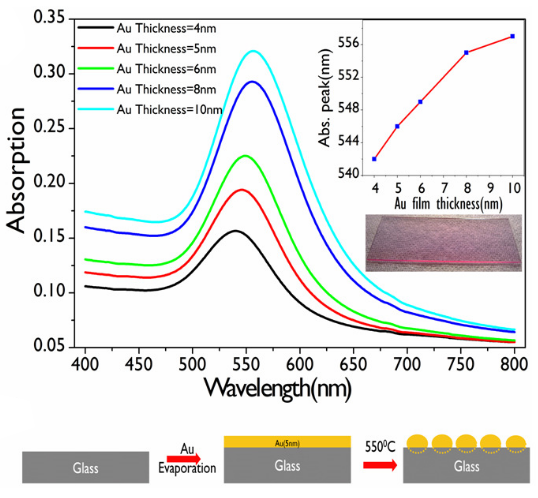
\includegraphics[width = .32\textwidth]{Moringthem/abs.png}
  \caption[Multipolar Contributions to the Scattered Electric Field]{ Decomposition of the  scattered electric field $\vb{E}^\text{sca}$ into its contributions  proportional to \textbf{a)} $a_1$,  \textbf{b)}  $b_1$, \textbf{c)} $a_2$ and \textbf{d)} $b_2$ [see Eq. \eqref{eq:EscaLC}] when a spherical particle (not shown) is illuminated by an $x$-polarized plane wave traveling in the $z$ direction. The scattered electric field $\vb{E}^\text{sca}$ is evaluated at a sphere larger than the particle: the arrow stream corresponds to the projection parallel to the evaluation sphere of $\vb{E}^\text{sca}$  and the color code corresponds to the magnitude of  $\vb{E}^\text{sca}$. A contour surface of the magnitude of $\vb{E}^\text{sca}$ is located at the center of each \textcolor{red}{coordinated system}. }
\label{fig:IncPapers}
\end{figure}


, as it can be seen in Fig. \ref{sfig:inc:1} where there are shown images of Transmission Electron Microscopy (TEM) of Au nanospheroids fabricated by thermal annealing by Meng et. al. \cite{meng_anisotropic_2015} where partially embedding  in the silica (SiO2) substrate of different degrees can be observed. While a larger incrustation degree of the meta-atoms decreases the overall sensing area of the metasurface, thus limiting its performance, a partial embedding in the substrate may be a desired feature for a biosensing-aimed metasurface since the greater its incrustation degree, the smaller the washability  of its meta-atoms due to the coupled microfluidics. 

 In


 One alternative to decrease a metasurface's washability is to partially embed it within the substrate while allowing the metasurface to still interact with the aqueous medium. 
 
 
 In this work, we study the optical response of a single partially embedded metallic nanosphere  and extend its behavior analytically into a disordered metasurface by employing an effective medium approach.





\begin{itemize}
	\item Objectives: What question are you answering with your work.\\
	\item Methology: What are your secondary goals so you achieve your objective. Also, how are you answering yout question: which method or model.\\
	\item Structure: How is this thesis divides and what is the content of each chapter.
\end{itemize}





















